\documentclass[11pt]{article}
\usepackage[T1]{fontenc}
\usepackage{amsthm,amsmath,amssymb,amsfonts,authblk,setspace}
\usepackage{xcolor}
\usepackage[colorlinks=true, allcolors=blue]{hyperref}
\usepackage{tikz}
\usepackage{pgfplots}
\pgfplotsset{compat=newest}
\usetikzlibrary{decorations.pathreplacing,angles,quotes}

\begin{document}

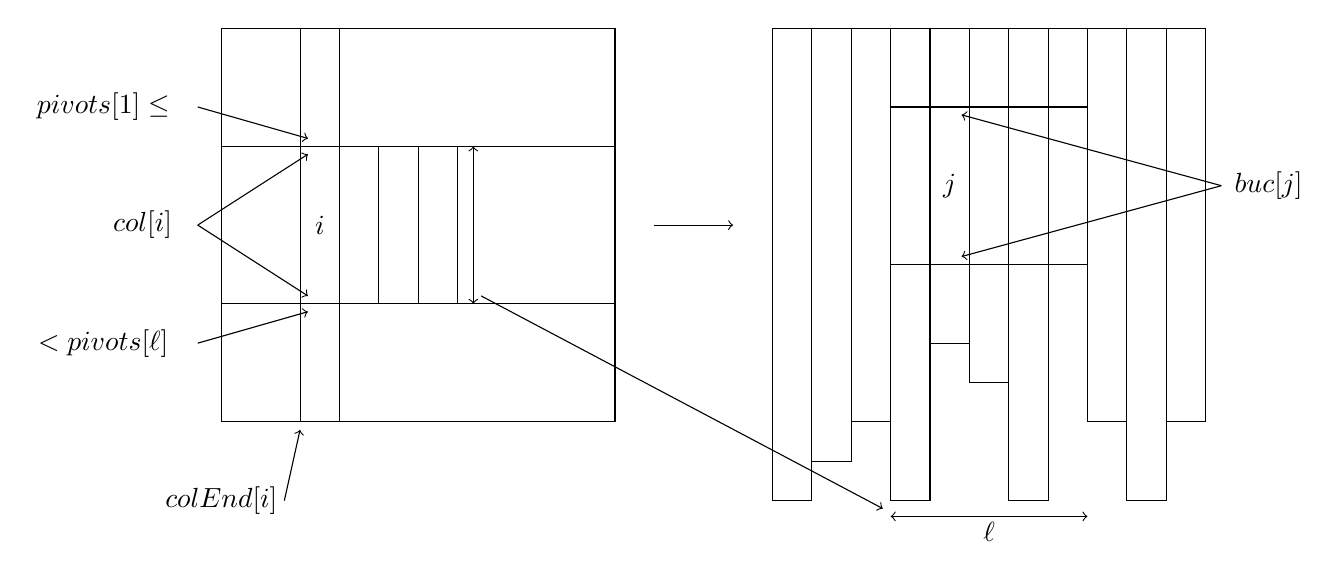
\begin{tikzpicture}%
\draw (-1.5,4) node {$pivots[1] \le$};
\draw (-1,2.5) node {$col[i]$};
\draw (-1.5,1) node {$< pivots[\ell]$};
\draw (1.25,2.5) node {$i$};
\draw (0,-1) node {$colEnd[i]$};
\draw [<->] (3.2,3.5) -- (3.2,1.5);

\draw [->] (-0.3,4) -- (1.1,3.6);
\draw [->] (-0.3,2.5) -- (1.1,3.4);
\draw [->] (-0.3,2.5) -- (1.1,1.6);
\draw [->] (-0.3,1) -- (1.1,1.4);
\draw [->] (0.8,-1) -- (1,-0.1); 

\draw (0,0) rectangle +(5,5);
\draw (0,1.5) rectangle +(5,2);
\draw (1, 1.5) rectangle +(0.5,2);
\draw (1, 0) rectangle +(0.5,5);
\draw (1.5, 1.5) rectangle +(0.5,2);
\draw (2, 1.5) rectangle +(0.5,2);
\draw (2.5, 1.5) rectangle +(0.5,2);

\draw [->] (5.5,2.5) -- (6.5,2.5);

\draw [->] (3.3,1.6) -- (8.4,-1.1);

\draw (9.75,-1.4) node {$\ell$};
\draw [<->] (8.5,-1.2) -- (11,-1.2); 
\draw (13.3,3) node {$buc[j]$};
\draw (9.25,3) node {$j$};
\draw [->] (12.7,3) -- (9.4,3.9);
\draw [->] (12.7,3) -- (9.4,2.1);

\draw (7,-1) rectangle +(0.5, 6);
\draw (7.5,-0.5) rectangle +(0.5, 5.5);
\draw (8,0) rectangle +(0.5, 5);
\draw (8.5,-1) rectangle +(0.5, 6);
\draw (9,1) rectangle +(0.5, 4);
\draw (9.5,0.5) rectangle +(0.5, 4.5);
\draw (10,-1) rectangle +(0.5, 6);
\draw (10.5,2) rectangle +(0.5, 3);
\draw (11,0) rectangle +(0.5, 5);
\draw (11.5,-1) rectangle +(0.5, 6);
\draw (12,0) rectangle +(0.5, 5);
\draw (8.5,2) rectangle +(0.5,2);
\draw (9,2) rectangle +(0.5,2);
\draw (9.5,2) rectangle +(0.5,2);
\draw (10,2) rectangle +(0.5,2);
\draw (10.5,2) rectangle +(0.5,2);
\end{tikzpicture}

\end{document}